%%%%%%%%%%%%%%%%%%%%%%%%%%%%%%%%%%%%%%%%%%%%%%%%%%%%%%%%%%%%%%%%%%%%%%%%%%%%%%
%%%%%%%%%%%%%%%%%%%%%%%%%%%%%%%%%%%%%%%%%%%%%%%%%%%%%%%%%%%%%%%%%%%%%%%%%%%%%%
%%
%% Dokumentacia k semestralnemu projektu z PRL
%%
%%%%%%%%%%%%%%%%%%%%%%%%%%%%%%%%%%%%%%%%%%%%%%%%%%%%%%%%%%%%%%%%%%%%%%%%%%%%%%
%%%%%%%%%%%%%%%%%%%%%%%%%%%%%%%%%%%%%%%%%%%%%%%%%%%%%%%%%%%%%%%%%%%%%%%%%%%%%%
\documentclass[11pt,a4paper,titlepage,final]{article}

% cestina a fonty
\usepackage[czech]{babel}
\usepackage[T1]{fontenc}
\usepackage[utf8]{inputenc}
% balicky pro odkazy
\usepackage[bookmarksopen,colorlinks,plainpages=false,urlcolor=blue,unicode]{hyperref}
\usepackage{url}
% obrazky
\usepackage[dvipdf]{graphicx}
% velikost stranky
\usepackage[top=3.5cm, left=2.5cm, text={17cm, 24cm}, ignorefoot]{geometry}
\usepackage{fancyhdr}

\begin{document}
\raggedright\large{\textbf{Projekt z predmetu PRL Martin Maga (xmagam00) \\Implementácie algoritmu Minimum extraction sort}}

\section{Teoretické rozobratie algoritmu}
Základná myšlienka tohto algoritmu je postavená nad binárnym stromom. V listových uzloch (listoch) sú uložené hodnoty, ktoré sa majú zoradiť. Každý nelistový uzol obsahuje procesor. Tento procesor je schopný porovnať hodnoty jeho 2 potomkov a menšiu z hodnôt, ktorú obdrží od svojich potomkov, uložiť do svojho uzlu. Tieto hodnoty postupne postupujú nahor po binárnom strome až nakoniec dorazia do koreňa, presne po "LOG (N) + 1 krokoch". Celý proces sa opakuje. Do koreňa sa ukladajú hodnoty vždy v 2 krokoch, najprv je hodnota uložená do koreňa (1.krok) a následne (2. krok) sa hodnota uloží do výstupné pola, kde sú hodnoty už zoradené.

Treba zdôrazniť, že strom je binárny, to znamená, že počet listov je mocnina 2. Preto je nutné zabezpečiť, že počet nezoradených hodnôt na vstupe musí byť nutne mocninou 2. Tento problém sa rieši, tak že sa doplní počet hodnôt na najbližšiu mocninu čísla 2 neutrálny číslom, napr. -1.
\section{Časová zložitosť}
Časová zložitosť tohto algoritmu je úzko spätá s priestorovou zložitosťou. Musíme si uvedomiť, že najmenšia hodnota v binárnom strome dosiahne koreň binárneho stromu po (log n) + 1 krokoch. Keď hodnota dosiahne koreň potrebuje 2 kroky a to 1. krok pre uloženie hodnoty a 2. krok na uloženie hodnoty do výstupnej zoradenej postupnosti. Následne sa zostávajúcich n - 1 hodnôt zo stromu odstráni a to v takom poradí, že sa odstráni od najmenšieho a to po 2 krokoch, opäť sa jedná odoslanie hodnoty do koreňa (1.krok) a odstránenie hodnoty z koreňa a uloženie do výstupnej postupnosti (2.krok). Keď spojíme vyššie spomenuté kroky tak dostane nasledujúcu zložitosť: 2 * (n – 1) + (log n) + 1. Po zjednodušení dostávame: 2 * n + log n – 1, čo je celkový počet krokov pre "n" hodnôt. Dominantná zložka v tomto vzorci je "n" preto je časová zložitosť algoritmu : t(n) = "O(n)", teda lineárna.

\section{Priestorová zložitosť}
V tomto algoritme používame binárny strom. Vieme ľahko určiť, že binárny strom potrebuje pre 8 hodnôt 8 listových uzlov. Keďźe tento strom je binárny každa z 2 hodnôt má 1 spoločného rodiča a ten rodič ďalšieho rodiča.
Vieme spočítať, že celkový počet úrovni(okrem listovej úrovne) je log (n) (logaritmus má základ 2). Rovnako vieme, že binárny strom obsahuje na každej vyššej úrovni o polovicu menej procesor až na úrovni koreňa, ktorý logicky obsahuje 1 uzol. Celkovo keď zrátame pre 8 hodnôt celkový počet uzlov dostaneme nasledovné: 1. úroveň - obsahuje 8 uzlov (najnižšia), 2. úroveň - obsahuje 4 uzly 3. úroveň  - obsahuje 2 uzly 4. úroveň (najvyššia) - 1 uzol (koreň). Celkovo obsahuje binárny strom pre zoradenie 8 hodnôt 15 procesorov. Pri skúmaní závislosti nad rôznym počtom vstupných hodnôt dostávame priestorovú zložitosť: p(n) = 2 * n - 1. (Počet procesorov)
\section{Celková cena algoritmu}
Celková cena algoritmu je: c(n) = p(n) * t(n). Pre náš algoritmus dostávame hodnotu: c(n) = (2 * n - 1) * n = $n^2$ (pri zanedbaní nejakých premenných). Celková cena riešenia je kvadratická, čo nie je optimálne pre paralelné riešenie. 

\section{Implementácia}
Pri implementácií algoritmu Minimum Extraction Sort bola použivá knižnica OpenMPI spolu s jazykom C. Táto knižnica umožňuje implementáciu algoritmov paralelne, pričom vytvára procesory (similuje ich), ktoré komunikujú prostredníctvom správ. Program mes.c po preložení paralelne vytvorí N procesorov podľa 2. parametru v skripte test.sh. Každý procesor si pri vytvorení uchová svoje jedinečné číslo, s ktorým ďalej pracuje. Celý algoritmus je spustení z koreňa, teda z procesora s $my_id$ s hodnotou 0. Tento procesor načíta vstupný súbor "numbers" a jednotlivé hodnoty následne prepošle listových procesorom. V koreňom procesore sa po načítaní vstupného súboru a odoslaní načítaných hodnôt jednotlivým procesorom skontroluje, že zadaný počet hodnôt je mocninou 2, pokiaľ nie je tak je hodnota doplnená na najbližšiu mocninu 2. Zvyšným listovým procesorom je odoslaná hodnota "-1", čo značí, že hodnota je nepoužitá, tj nebude sa nachádzať vo výstupnej zoradenej postupnosti. 

Celý algoritmus pokračuje obdržaním hodnôt od koreňa stromu a jej uložením do pomocnej premennej.Následne sa realizuje nekonečný cyklus. V tomto cykle sa postupne realizuje nasledovné. Pre každý ne-koreňový a zároveň listový procesor sa zistí id procesory jeho rodiča(v závislosti od jeho aktuálneho $my_id$). Ten pošle hodnotu svojho čísla rodičovi a prijme hodnotu od rodiča. Pokiaľ nejaký uzol dostane od rodiča hodnotu "-1", znamená,  že svoju uloženú hodnotu poslal už svojmu rodičovi a zároveň táto hodnota bola zároveň menšia ako hodnota jeho brata a teda môže svoju činnosť skončiť, keďže je listový. Preto sa aj procesor následne ukončí. Treba podotknúť akým spôsobom sa pracuje s premennou $"my_id"$, ktorá obsahuje jedinečné číslo pre každý procesor. Hodnota 0 predstavuje koreň stromu, hodnoty 1 - ((počet zadaných procesorov + 1) / 2) - 2 sú hodnoty nelistových procesorov a hodnoty ((počet zadaných procesorov + 1) / 2) - 1 až počet zadaných procesorov predstavuje listové procestory.

Pre každý nelistový procesor sa zistí, od ktorých procesorov (potomkov) má získať hodnoty. Ten získa obe hodnoty a menšiu z nich si uloží a prepošle svojmu rodičovu (opäť k výpočtu rodiča použije hodnotu $my_id$). Väčšiu hodnotu pošle späť svojmu potomkovi, od ktorého ju održal a potomkovi, od ktorého získal menšiu hodnotu pošle hodnotu "-1" na ukončenie.  Tento proces sa neustále opakuje pokiaľ procesor nie je ukončený, tj neobdržal hodnota -1 od svojho rodiča. Ako postupne hodnoty postupujú až dosiahnu koreň. Ten postupne vypisuje hodnoty, ktoré obdržal na výstup a pošle sa hodnota "-1" nelistovému procesoru, od ktorého obdržal menšiu hodnotu a druhému potomkovi pošle hodnotu späť. Až nakoniec sám obdŕži hodnotu -1 => všetky ostatné procesory sú ukončené a sám sa ukončí.


\section{Komunikačný protokol}
Na nasledujúcom obrázku je zobrazený komunikačný protokol:
 \begin{figure}[h]

\begin{center}
\scalebox{0.15}{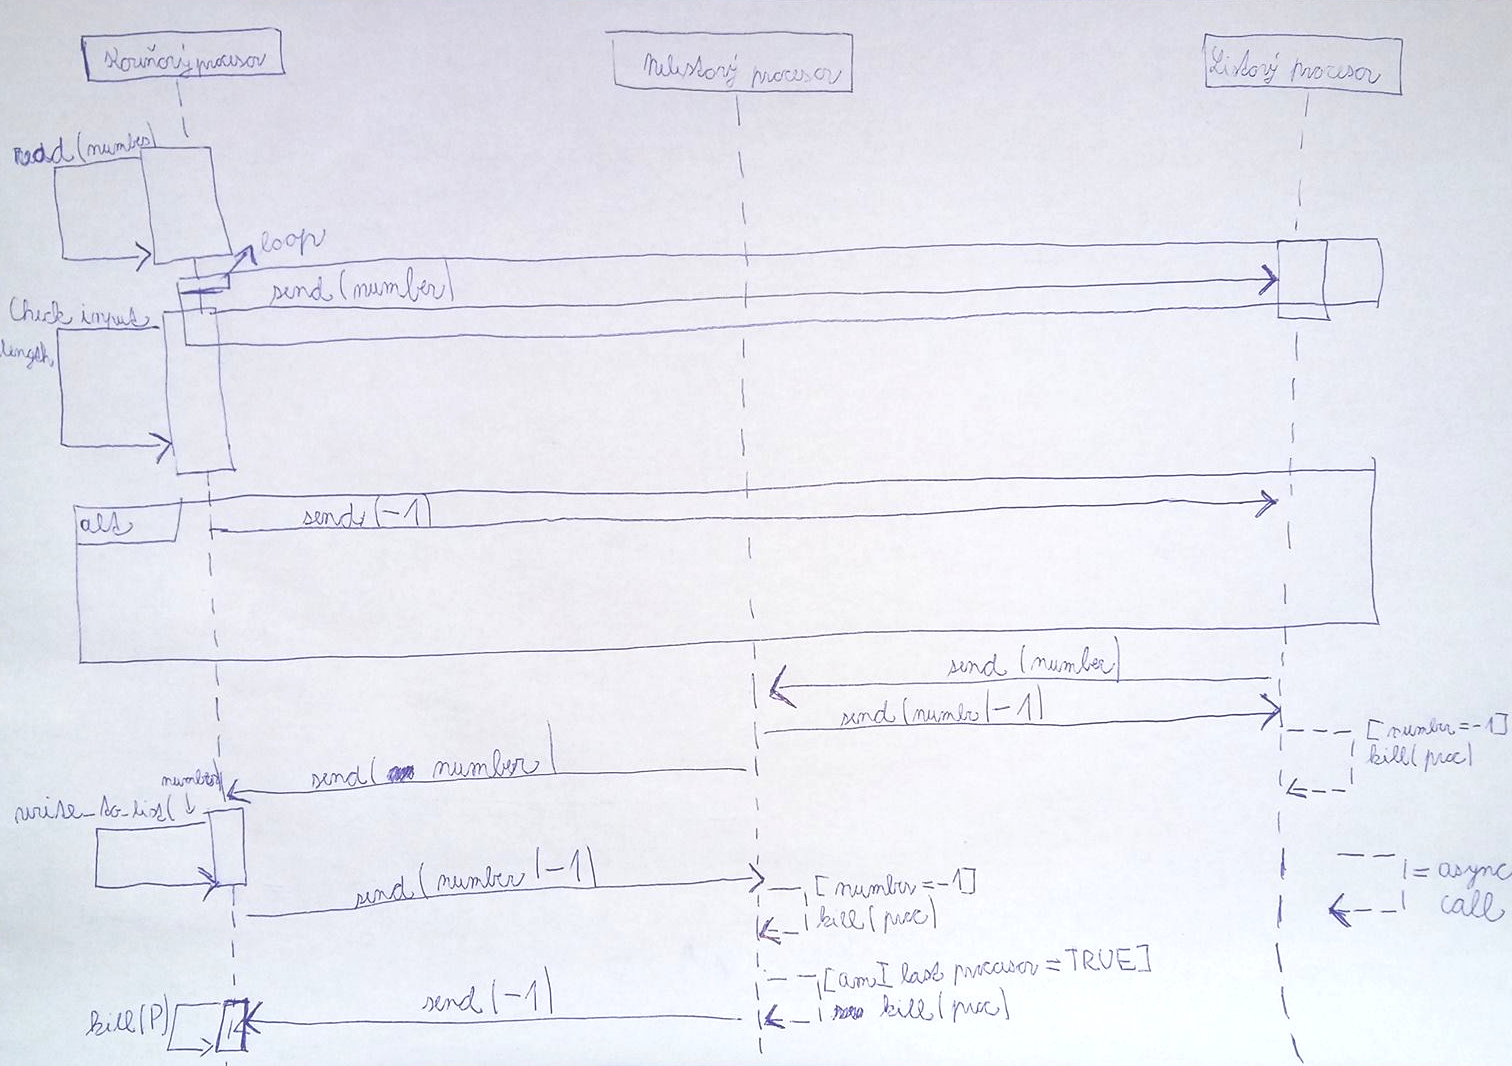
\includegraphics{img/diagram.eps}}
\caption{Sekvenčí diagram popísujúci komunikáciu}
\end{center}

\end{figure}


\section{Experimenty}
V tejto kapitole sme overovali časovú zložitosť, ktorá je približne lineárna. Z tohto môžme predpokladať, že výsledný graf bude mať tvar priamky. Pre overenie sme vykonali experiment nasledovne: Ako vstup sme postupne spúštali skript test.sh nasledovne: 1. beh test.sh 2 3 2. beh test.sh 4 7 3. beh test.sh 8 15.

Algoritmus sme spúštali na serveri merlin(Linux merlin.fit.vutbr.cz 3.12.56 $x86\_64$ GNU/Linux). Pre správnosť výsledkov sme každú konfiguráciu spustili 100x a výsledný čas som spriemeroval. Treba spomenúť, že nebolo možné overiť riešenie pre väčší počet hodnôt, keďže server merlin nedovoluje spustiť program s väčším počtu procesorov.

Z implementačného hľadiska treba podotknúť, že meranie je realizované funkcou $"MPI_Wtime()"$, ktorá vracia počet sekúnd. Tento funkcia sa volá na začiatku a na konci pre koreňový procesor.
 \begin{figure}[h]

\begin{center}
\scalebox{0.5}{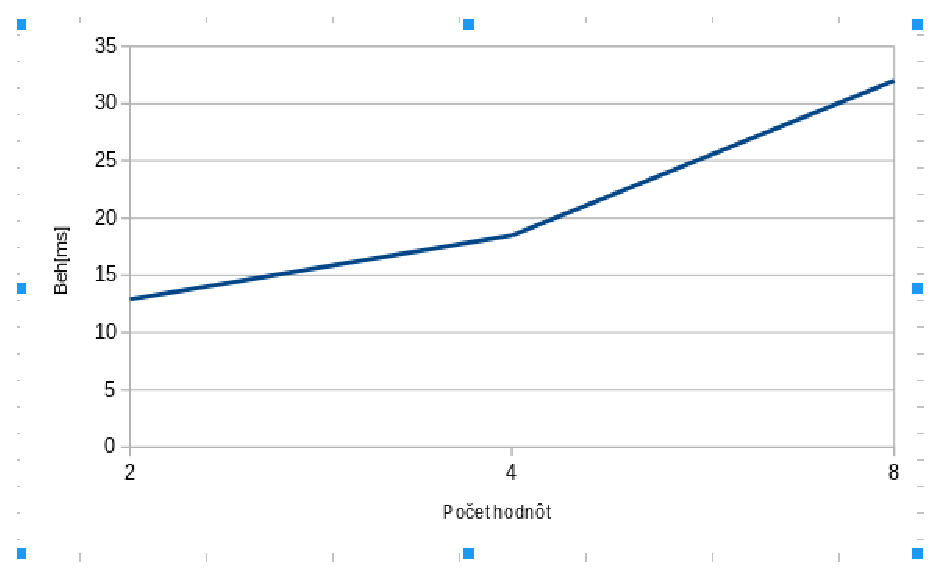
\includegraphics{img/mes.eps}}
\caption{Graf časovej závislosti počtu vstupných hodnôt a behu programu v ms}
\end{center}

\end{figure}

\section{Záver}
Implementovali sme algoritmus Minimum Extraction Sort s knižnicou OpenMPI. Rovnako sme odvodili teoretickú časovú, priestorovú a celkovú zložitosť algoritmu, ktorú sme experimentom aj potvrdili.
\end{document}



